\chapter{Evaluation}
\label{chap:evalution}

% questions to answer
% - how do the runtimes compare to each other?
% - how do the runtimes compare to native code?
% - which set of wasm modules are chosen for the benchmarks and why?
% - what programming languages are chosen for the benchmarks and why?
% - what are the results of the benchmarks?
% - what are the limitations of the benchmarks?


\section{Methodology}
\label{sec:methodology}

\subsubsection{Microbenchmarks}

\subsubsection{Macrobenchmarks}

\subsection{Goals}
\label{subsec:goals}

\section{Setup}
\label{sec:setup}

% TODO: add a diagram of the setup

\subsection{Programming Languages}
\label{subsec:programming-languages}

\section{Benchmarks}
\label{sec:benchmarks}

\subsection{Cold Start - Instantiation}
\label{subsec:cold-start}

\begin{figure}[htbp]
    \centering
        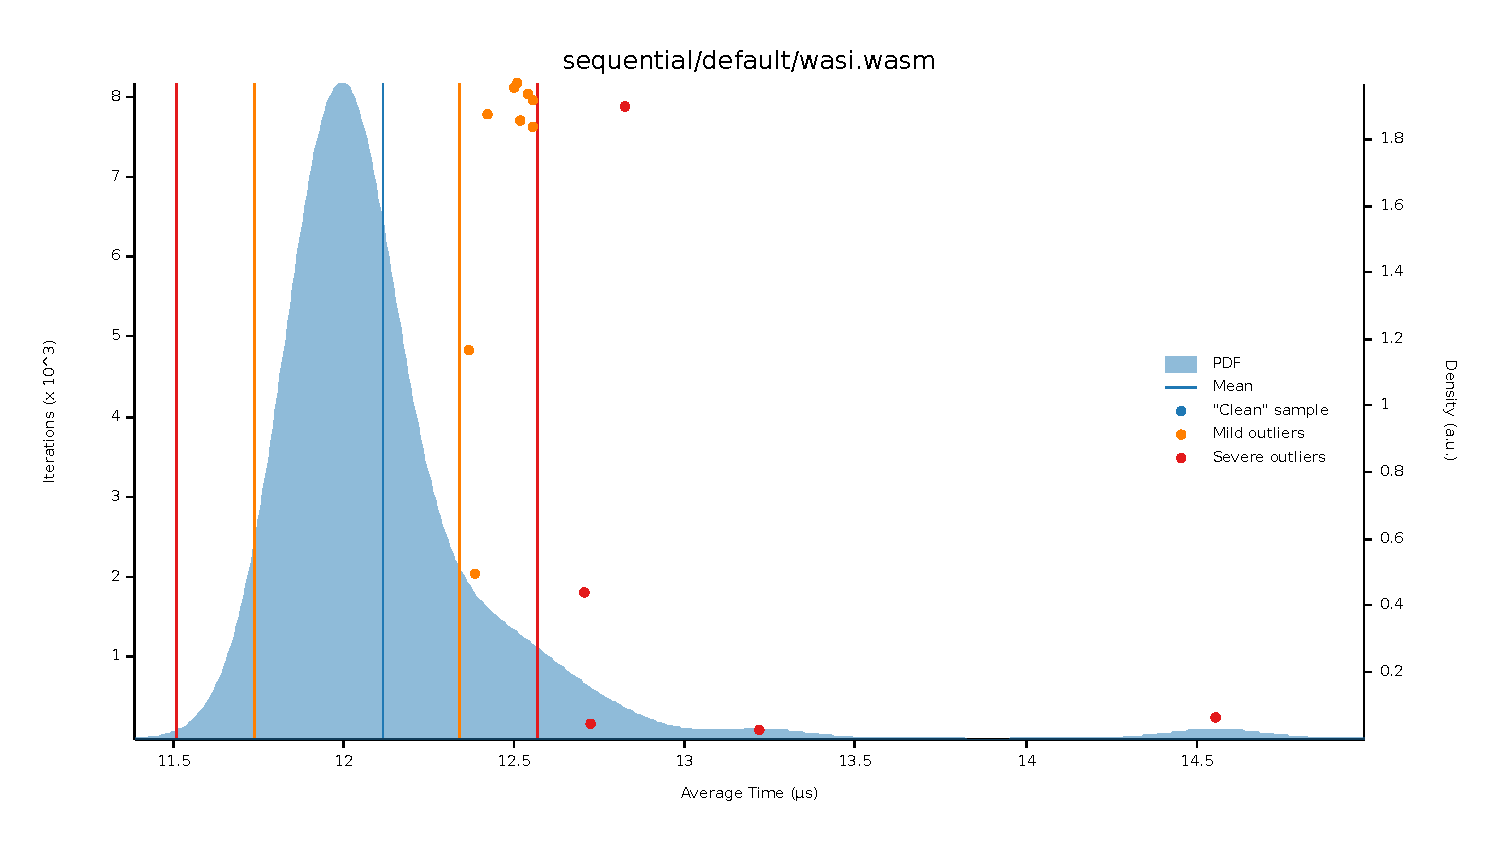
\includegraphics[width=1\linewidth]{images/benches/sequential_default_wasi.pdf}
    \caption{Instantiation distribution of a WASI module with Wasmtime}
    \label{fig:bench:instantiation:wasi}
\end{figure}

\begin{figure}[htbp]
    \centering
        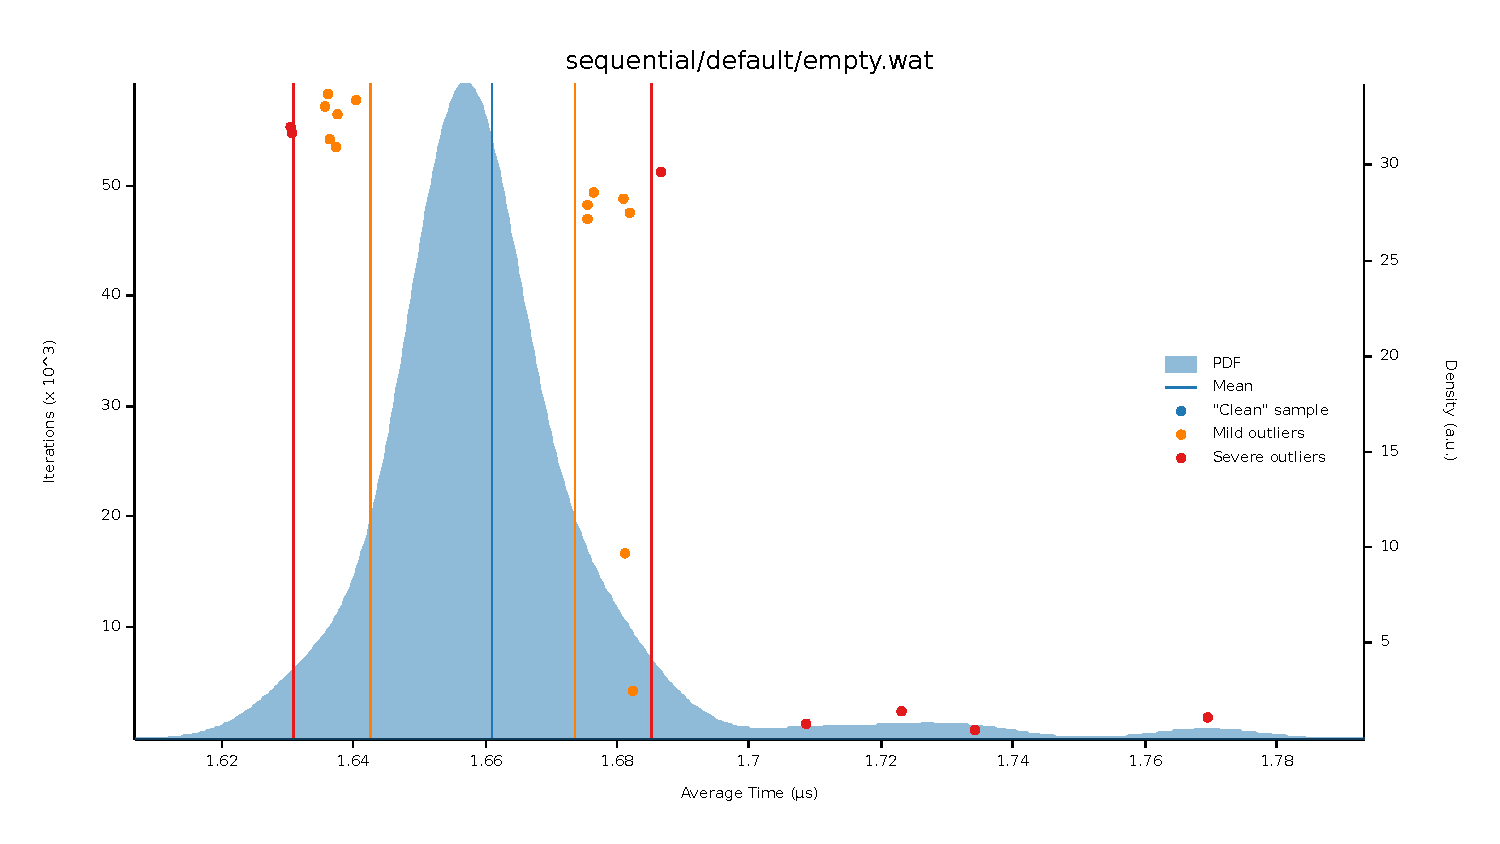
\includegraphics[width=1\linewidth]{images/benches/sequential_default_empty_wasm.pdf}
    \caption{Instantiation distribution of an empty Wasm module with Wasmtime}
    \label{fig:bench:instantiation:empty-wasm}
\end{figure}
